\begin{figure}[htbp]
\centering
\captionsetup{
  justification=raggedright,
  labelsep=none,
  singlelinecheck=false,
  labelformat=boldlabel,
}
\caption[Figure 5: \footnotesize ]{\footnotesize \textbf{: Average portfolio characteristics over time.} Weighted-average stock characteristics of each ML-ensemble portfolio (sum of end-of-period portfolio weights times the characteristic) at every rebalance date. Each panel is one characteristic: Sharpe ratio (12m), earnings yield (NI/ME), return on equity (12m), gross profitability (GP/AT), dividend yield (36m median), return volatility (12m), log market capitalization, quality minus junk (QMJ) and the three-year change in FCF/BE. Each line is one portfolio-construction scheme (RP, RP\_BOX, HRP, CS, SW, EW, MVO, MVO\_BOX); the dashed black line is the IBOV benchmark's weighted average. Vertical scales differ across panels.}
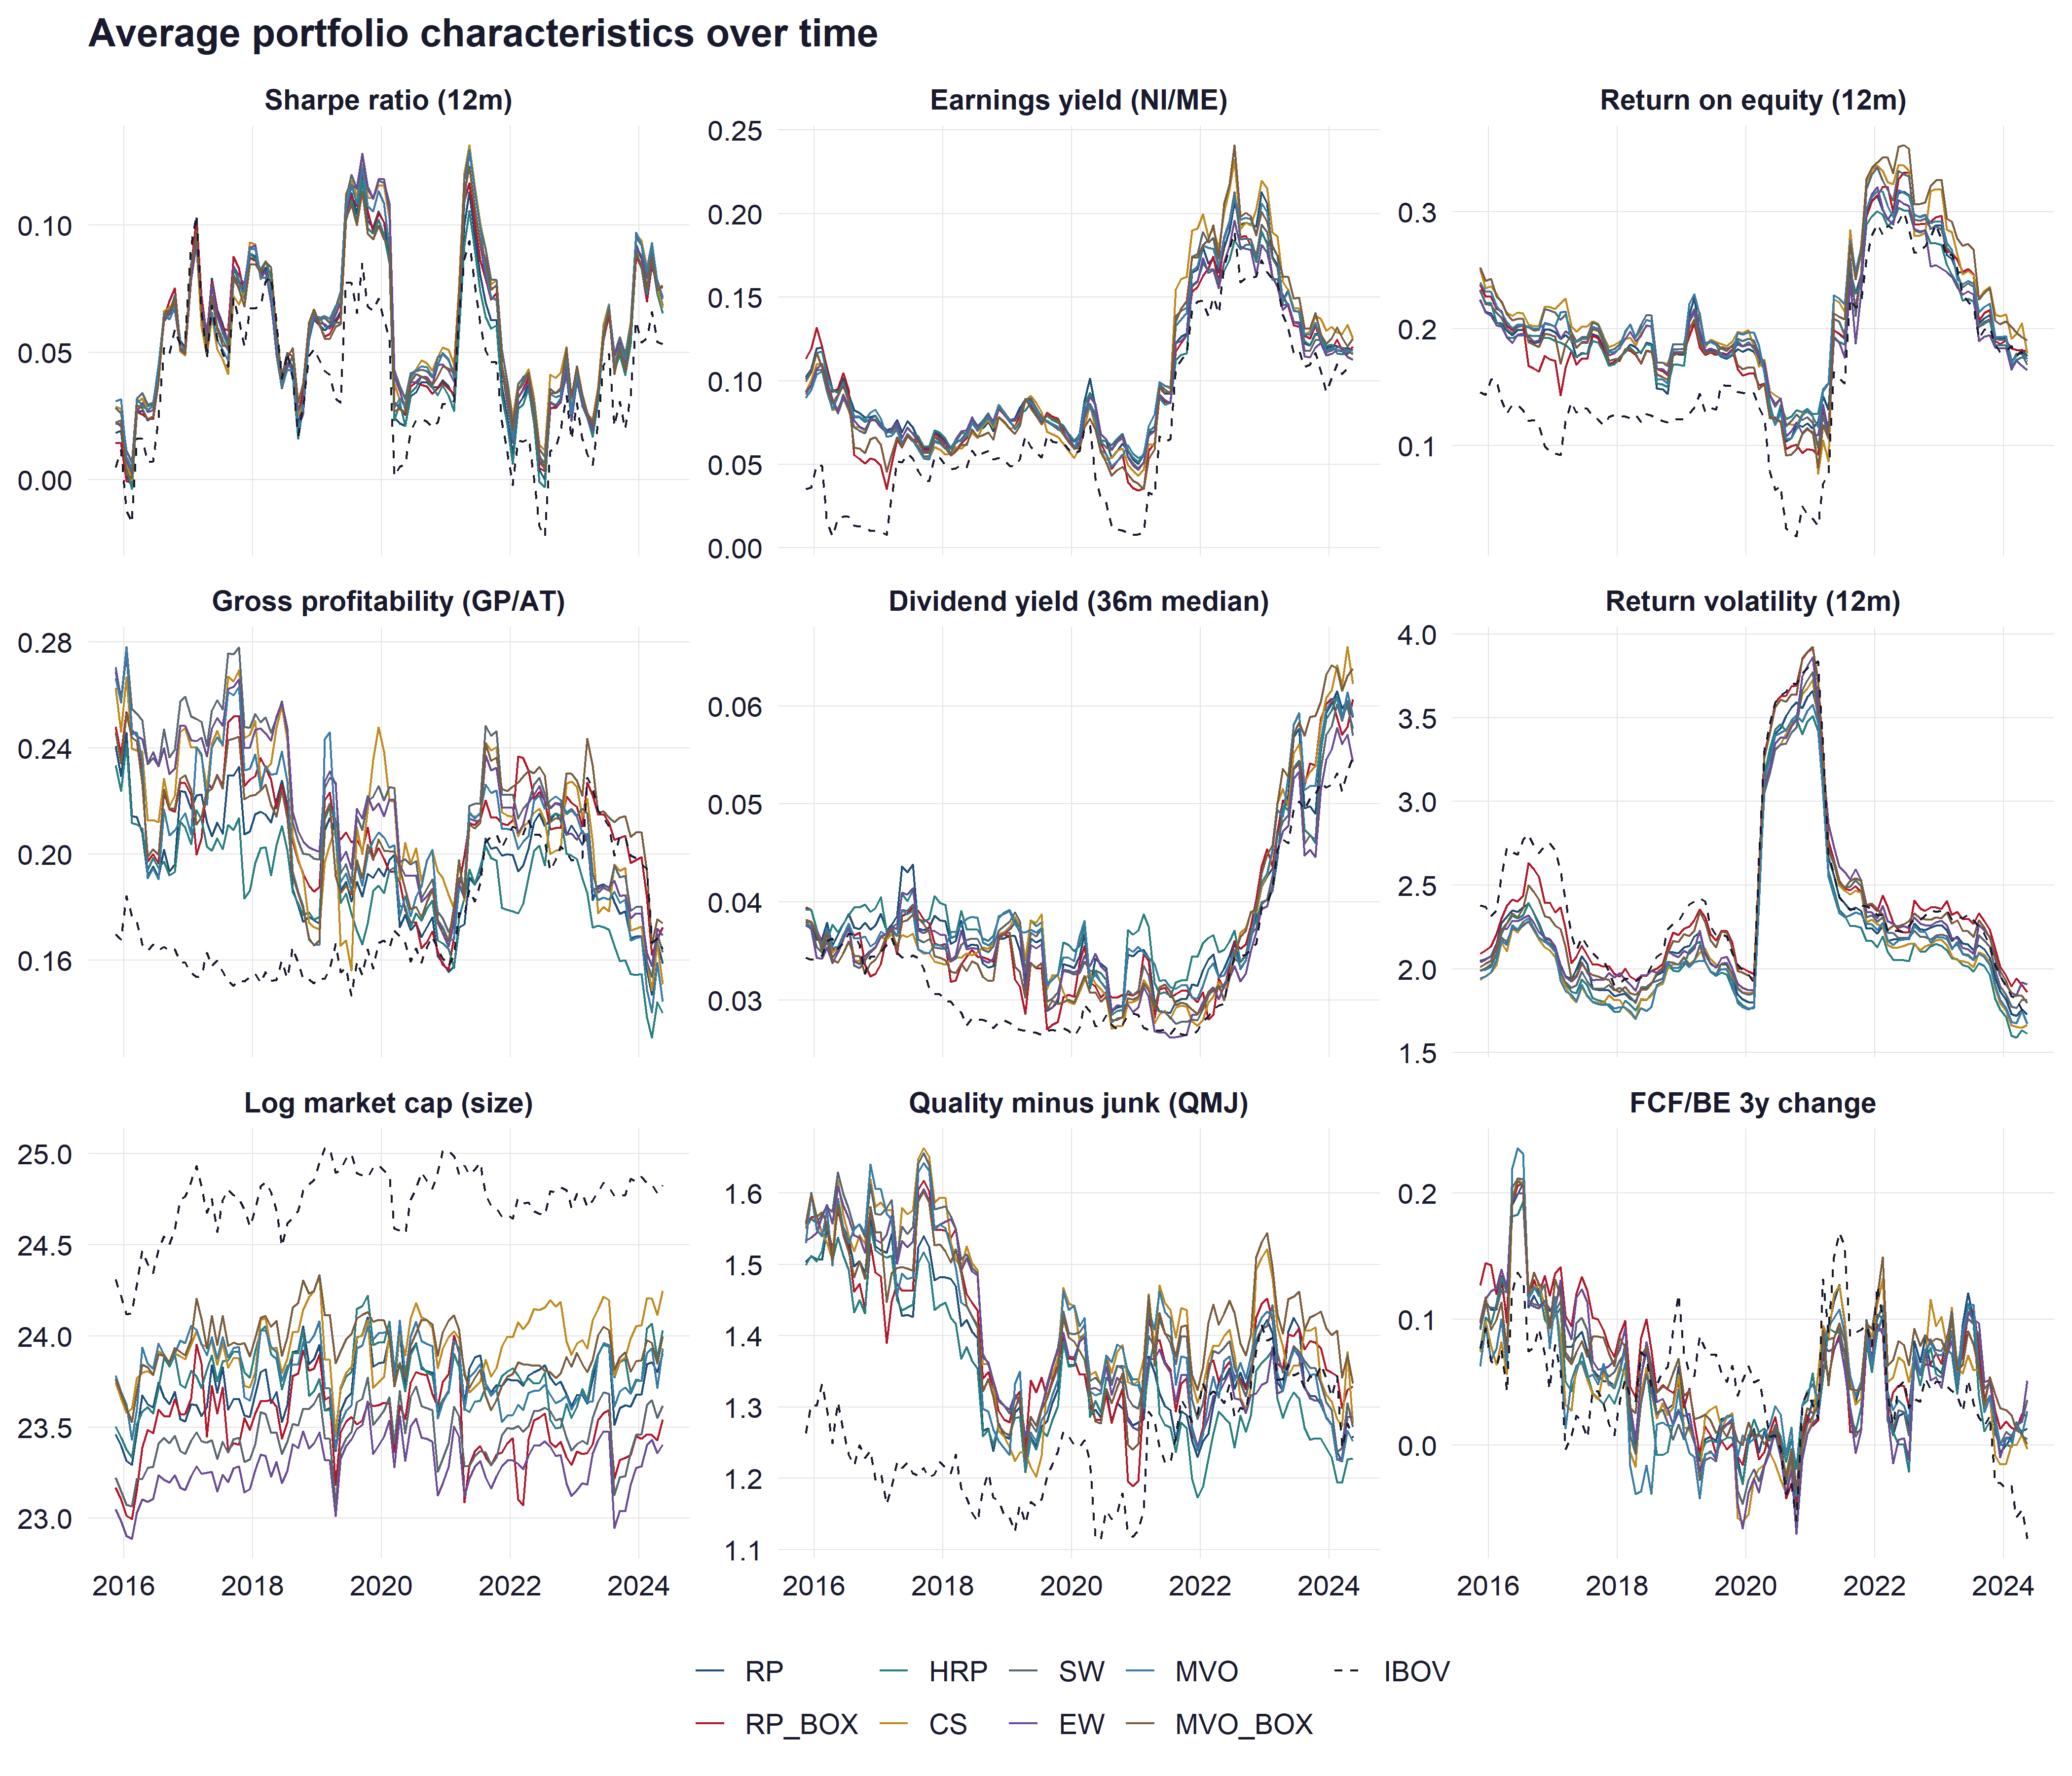
\includegraphics[width=\linewidth]{figures/portfolio_characteristics.png}
\label{fig:port_char}
\end{figure}
